\documentclass[twoside]{article}
\input{ISC18-english.sty}
%%%%%%%%%%%%%%%%%%%%%%%%%%%%  Make sure to compile twice for proper cross-references. %%%%%%%%%%%%%%%%%%%%%%%
%%%%%%% For proper display of references, compile the document twice. %%%%%%%%%%%%%%%%%%%%% 
%%%%%%%%%%%%%%% If using TeX Live, compile using pdflatex command %%%%%%%%%%%%%%%%%%%%%%%
\begin{document}
\thispagestyle{empty}
%%%%%%%%%%%%%%%%% Article title header  %%%%%%%%%%%%%%%%%%%%
\fancyhead[LE]{Solvency Ratio and Insurance Policy Sales}
%%%%%%%%%%%%%%%%% Article authors header   %%%%%%%%%%%%%%%%%%%%
\fancyhead[RO]{R. Mahmoudvand}
\begin{center}
{
\includegraphics [height=25mm, width=150.3mm] {Images/isc18E}} \\
\vspace*{-1.8cm}
%\begin{center}
%\color{blue} 
%{\hspace{0.1cm}\rule{\textwidth}{1mm}}\\
%\end{center}
\vspace*{4cm}
%%%%%%%%%%%%%%%%% Article title  %%%%%%%%%%%%%%%%%%%%
{\Large \bf Investigating the Relationship between Iranian Insurance Companies' Solvency Ratio and Insurance Policy Sales}\\
%%%%%%%%%%%%%%%%% Article authors and affiliations %%%%%%%%%%%%%%%%%%%%
{\bf
Rahim Mahmoudvand$^1$  \footnote[1]{{\bf Corresponding Author:} {\tt r.mahmoudvand@basu.ac.ir }} \\
$^1$Department of Statistics, Bu-Ali Sina University, Iran} \\
\end{center}
\rule{\textwidth}{0.2mm}\\
%%%%%%%%%%%%%%%%% Article abstract  %%%%%%%%%%%%%%%%%%%%
\noindent{\bf Abstract:}\\
The Central Insurance of Iran introduced the financial solvency ratio as a supervisory tool for insurance companies following the approval of Regulation No. 69 in February 2012. This metric assesses an insurer's financial capacity to cover accepted risks and classifies companies into five levels, with Level 1 (ratio above 100\%) considered desirable. Despite regulatory flexibility regarding remedial actions, market perception increasingly associates higher solvency ratios with insurer reliability. This paper examines whether the annual publication of solvency ratios influences insurance policy sales. Using data from 16 Iranian insurance companies spanning 2012-2024, we construct a "co-movement" index to measure the directional alignment between solvency ratio changes and subsequent year premium writings. Our methodology accounts for the inherent time lag in consumer response and addresses non-stationarity concerns in time series data. The findings provide preliminary evidence on the market discipline role of solvency disclosure in Iran's insurance industry.
 
\noindent{\bf Keywords:} 
Solvency Ratio, Insurance Regulation, Market Discipline, and Policy \\
\noindent{\bf Mathematics Subject Classification (2010):} $\rm 62P05$, $\rm 91B30$, $\rm 62H20$. \\
\hspace{1cm}\rule{\textwidth}{0.2mm}\\
%%%%%%%%%%%%%%

\section{Introduction and Overview}

The Central Insurance of Iran introduced financial solvency as a supervisory tool for insurance companies during the 2010s. This instrument measures an insurance institution's financial capacity to cover accepted risks. To operationalize this concept, Regulation No. 69 was approved in February 2012, and the solvency ratio index has been calculated and reported since 2012. The solvency ratio is obtained by dividing the available capital by the required capital and, according to the provisions of the solvency regulation, is classified into five levels. Among these five levels, only Level 1, which includes values exceeding 100\%, is considered desirable. Companies falling into other levels with ratios below 100\% must undertake various remedial measures. When the solvency ratio falls below 70\%, among the proposed actions, a reduction in policy issuance (Article 12 of Regulation No. 69) is mentioned. Although according to Article 12, insurance companies may not implement this measure, what has been promoted in the media and among policyholders is that an insurance institution with a higher solvency ratio is more suitable for purchasing insurance policies.

The theoretical foundation for this relationship stems from the market discipline hypothesis, which suggests that public disclosure of risk information influences both consumer behavior and management actions. Meier (2006) examine the determinants of policyholder behavior and find that financial strength indicators significantly influence surrender decisions and purchasing patterns in life insurance markets. This finding is particularly relevant to emerging insurance markets where information asymmetry between insurers and policyholders remains significant. Furthermore, Pasiouras and Gaganis (2013) investigate the relationship between regulatory pressure and insurance company performance across multiple countries, demonstrating that solvency requirements create market-based incentives for financial soundness that extend beyond mere compliance.

The effectiveness of solvency regulation depends crucially on whether disclosed information influences stakeholder decision-making. Cummins and Phillips (2005) analyze the relationship between insurer financial strength and market demand, finding that capitalization levels affect premium growth and market share. Their research demonstrates that consumers respond to financial strength information, directing purchases toward better-capitalized insurers, thereby creating natural market discipline. Additionally, Hanika (2025) examines market discipline in life insurance and concludes that public risk disclosure encourages less risky management actions, as insurers act to maintain higher solvency ratios to mitigate adverse policyholder reactions.

The informational signals transmitted within the market may suffer from credibility deficits if stakeholders cannot effectively utilize disclosed solvency information in their decision-making processes. Therefore, in this note, we aim to investigate whether the annual reporting of this ratio has had any relationship with policy sales. Specifically, we examine whether consumers respond to solvency information by directing their purchases toward companies with stronger solvency positions, thereby creating market-based incentives for financial soundness.

\section{Data and Methodology}

\subsection{Data Description}

For this investigation, we have two variables: the solvency ratio and policy issuance. We need these variables over time and disaggregated by insurance companies. The solvency ratio, as a supervisory tool of the Central Insurance for assessing the financial solvency of insurance institutions, was calculated and reported immediately after the approval of Regulation No. 69 for the year 2012. However, time series of this ratio for the entire period from 2012 to 2025 are not available in the statistical databases of the Central Insurance. Therefore, multiple sources were used to compile the solvency ratio time series for the mentioned period through their combination.

Additionally, policy issuance data for this period disaggregated by companies were not available as time series, necessitating the extraction of policy issuance data by insurance companies from several statistical yearbooks of the Central Insurance. In this note, due to lack of access to complete statistics, not all insurance companies were examined, but according to the introduced approach, interested parties can conduct further studies in this area. The companies studied include: Alborz, Asia, Dana, Dey, Iran, Karafarin, Kowsar, Mellat, Mihan, Moalem, Novin, Parsian, Razi, Saman, and Sina.

\subsection{Methodological Approach}

An important point in examining these data is the time lag in the existence of a relationship between the two variables under study. Simply put, when the solvency ratio for 2012 is reported, its effect is not seen in the issuance statistics of 2012 but rather in times after 2012. Therefore, we placed the solvency ratio for the period 2012 to 2023 against policy issuance for the period 2013 to 2024.

Another point that should be considered in this investigation is the time dependence of the data. Given that in time series, there may be no stationarity in mean and variance, using indices such as the Pearson correlation coefficient (due to dependence on mean and variance) can be misleading. Therefore, we use simpler indices. In this note, we prefer to use a simple index that only measures the direction alignment of changes in the two series of solvency ratio and policy issuance.

For this purpose, if for two consecutive years the direction of change in both series is the same, we assign a positive one, otherwise zero. The proportion of periods in which these two series have changed in the same direction is introduced as the mentioned index. Mathematically, if $X_t$ is the solvency ratio at time $t$ and $Y_t$ is the number of policy issuances at time $t$, then the proposed index is as follows:

\begin{equation}
\bar{C} = \frac{1}{T-1}\sum_{t=1}^{T-1} \mathbb{I}\{D_t^X \cdot D_{t+1}^Y > 0\} > 0 \}
\end{equation}

where $I\{\cdot\}$ is the indicator function and $D_t^z=Z_t-Z_{t-1}$. This index is somewhat similar to Kendall's correlation coefficient. Given the calculation method of this index, we can consider the name "co-movement" for it.


\section{Findings}

The co-movement index values were calculated for the 16 companies under investigation over the period 2012 to 2023 (with policy sales data extending to 2024). The values were sorted in ascending order and are displayed in Figure 1. As observed, the index values for the 16 companies under investigation range from approximately 0.18 to 0.73. Furthermore, the companies have been classified into six categories based on their co-movement levels. The classifications are presented in Table 1.

\begin{table}[h]
\centering
\caption{Classification of Insurance Companies by Co-movement Index Levels}
\label{tab:classification}
\small
\begin{tabular}{|c|l|c|l|}
\hline
\textbf{Category} & \textbf{Company} & \textbf{Co-movement Index} & \textbf{Interpretation} \\
\hline
1 & Moalem & 0.18 & Strong inverse co-movement \\
\hline
2 & Alborz & 0.27 & Relatively strong inverse co-movement \\
\hline
3 & Parsian, Mihan, Karafarin & 0.45 & Random co-movement \\
\hline
4 & Razi, Mellat, Kowsar, Iran, Asia & 0.54 & Random co-movement \\
\hline
5 & Pasargad, Novin, Dey & 0.64 & Noticeable co-movement \\
\hline
6 & Sina, Saman, Dana & 0.73 & Relatively strong co-movement \\
\hline
\end{tabular}
\end{table}

The results reveal considerable heterogeneity in the relationship between solvency ratios and policy sales across Iranian insurance companies. For companies in the first and second categories (Moalem and Alborz), the negative co-movement values indicate that improvements in solvency ratios were paradoxically associated with declines in policy sales, or conversely, deteriorations in solvency coincided with increased sales. This counter-intuitive pattern may reflect unique market positioning, brand loyalty factors, or specific marketing strategies that override solvency considerations for these particular insurers.

The third and fourth categories, comprising eight companies with index values around 0.45-0.54, exhibit what can be characterized as random co-movement. These values, hovering near 0.5, suggest no systematic directional relationship between solvency ratio changes and subsequent policy sales. For these insurers, solvency disclosures appear to have minimal impact on consumer purchasing decisions, with other factors likely dominating the sales dynamics.

The fifth and sixth categories, including seven companies with index values ranging from 0.64 to 0.73, demonstrate positive and meaningful co-movement. Particularly notable are Sina, Saman, and Dana in the sixth category with a relatively strong co-movement value of 0.73. For these companies, improvements in solvency ratios are consistently followed by increases in policy sales in the subsequent year, suggesting that consumers indeed respond to solvency information by directing their purchases toward financially stronger insurers.

\begin{figure}[h]
\centering
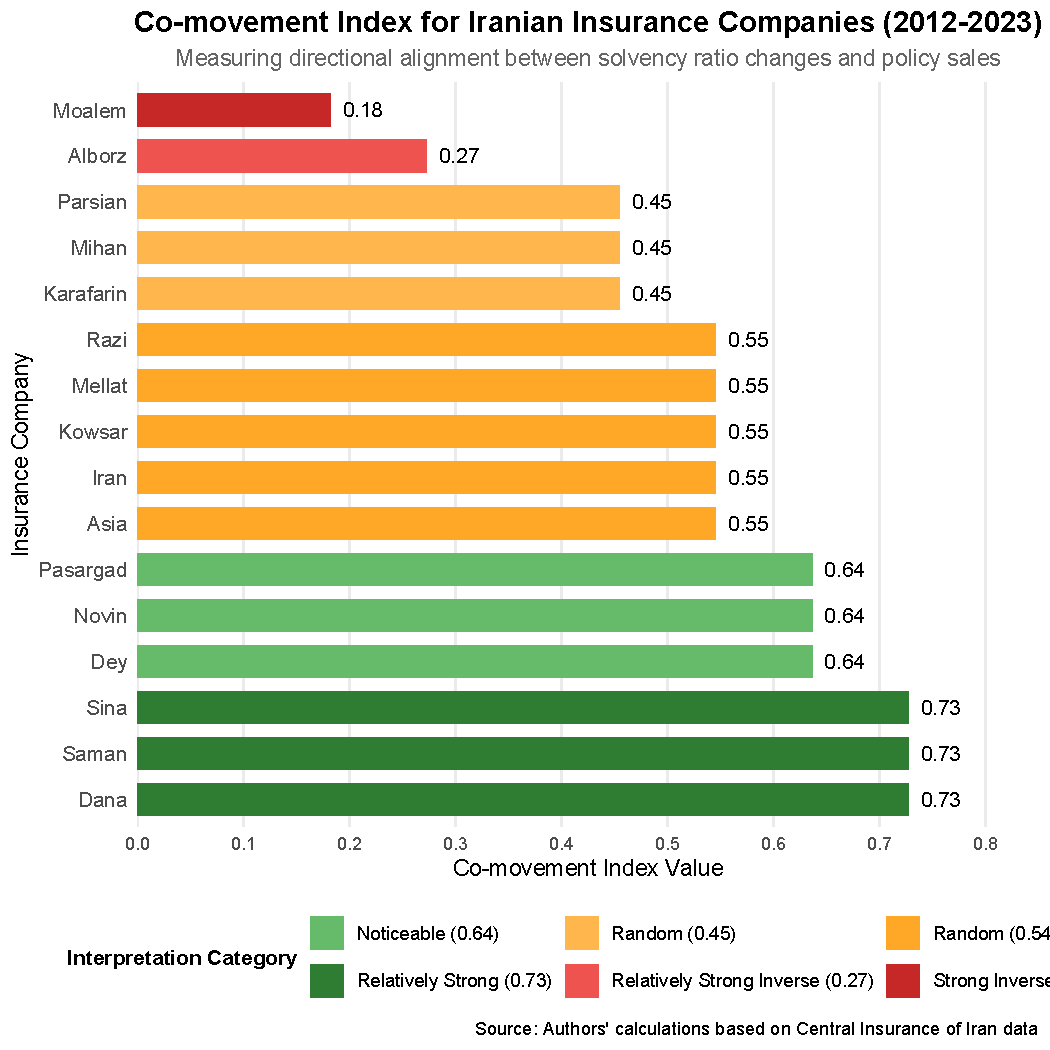
\includegraphics[width=\textwidth]{Images/co_movement.pdf}
\caption{Co-movement Index for Companies under Investigation (2012-2023)}
\label{fig:comovement}
\end{figure}

\subsection{Statistical Inference for the Co-movement Index}

To assess whether observed co-movement values differ significantly from random chance, we can derive the sampling distribution of $C$ under the null hypothesis of independence. Let $p$ be the true probability of directional alignment. Under the null hypothesis $H_0: p = 0.5$, the number of concordant directional changes $C = \sum_{t=1}^{T-1} \mathbb{I}\{D_t^X \cdot D_{t+1}^Y > 0\}$ follows binomial distribution  $\text{B}(T-1, 0.5)$.

This allows construction of approximate confidence intervals. However, given our limited time span, exact binomial confidence intervals are preferable. For a company with $\bar{c} = 0.73$ (8 concordant changes out of 11), the 95\% confidence interval based on the binomial distribution is approximately [0.39, 0.94]. This width highlights the uncertainty inherent in short time series and suggests caution in overinterpreting individual company values.

To test whether the co-movement index differs significantly from 0.5, we can compute the exact p-value:
%
\begin{equation}
p\text{-value} = 2 \times \min\left[ P(C \leq c), P(C \geq c) \right]
\end{equation}
%
where $c$ is the observed number of concordant changes. For $c = 8$ ($\bar{c} = 0.73$), $P(C \geq 8) = \sum_{k=8}^{11} \binom{11}{k} 0.5^{11} \approx 0.113$, yielding a two-sided p-value of approximately 0.226, indicating that this value does not reach conventional significance levels given the limited sample size. The co-movement index of $\bar{c}=0.18$ for Moalem Insurance Company yields a p-value of approximately 0.065, suggesting that the inverse relationship is statistically significant at the 10\% level (though not at the conventional 5\% level). 

%\subsection{Limitations}

%This study has several limitations that should be acknowledged. First, the incomplete availability of data prevented the inclusion of all insurance companies operating in Iran. Second, our co-movement index, while robust to non-stationarity, captures only directional relationships and not the magnitude of effects. Third, other factors influencing policy sales, such as pricing strategies, marketing efforts, and brand reputation, are not controlled for in this simple bivariate analysis. Future research should extend this work using panel data econometric approaches that can account for company-specific heterogeneity and additional control variables \cite{naseri2024early}.

\section{Conclusion}

As discussed, the solvency ratio of insurance companies is used by the Central Insurance as a supervisory tool and, according to the proposed classification, leads to various conclusions. When the ratio falls below 70\%, one of the corrective measures relates to reducing policy issuance, although companies may pursue measures other than this. However, the image of this ratio in the minds of policyholders is negative, and it is expected that companies with lower solvency ratios receive less chance in insurance policy purchases.

With this explanation, this note examined the statistical relationship between the solvency ratio and the number of policy issuances in 16 Iranian insurance companies from 2012 to 2023. Among the results, for companies such as Moalem and Alborz, we observe an inverse co-movement, meaning that with an increase or decrease in the solvency ratio, insurance sales statistics have changed in the opposite direction. This finding challenges the assumption that solvency information uniformly influences consumer behavior and suggests that for some insurers, other factors such as brand reputation, distribution channels, or pricing strategies may dominate purchasing decisions.

In contrast, for companies such as Dana, Sina, and Saman, the alignment between the solvency ratio and changes in insurance sales statistics has been direct and relatively strong. These companies, with co-movement indices of 0.73, demonstrate that their policyholders are responsive to solvency disclosures, directing their purchases toward the insurer when its financial position strengthens. This pattern is consistent with the market discipline hypothesis and suggests that solvency disclosure can create positive incentives for insurers to maintain strong capital positions.

For some companies, it appears that there is no relationship between the solvency ratio and sales statistics. The eight companies in the third and fourth categories, with index values around 0.45-0.54, exhibit essentially random relationships. This finding may indicate that solvency information is either not effectively communicated to policyholders of these companies, or that policyholders do not consider this information material to their purchasing decisions when selecting among these insurers.

The heterogeneity observed across companies suggests that the effectiveness of solvency disclosure as a market discipline mechanism depends on company-specific factors including brand perception, customer demographics, distribution channels, and the extent to which solvency information is publicized and understood by consumers. Companies with strong positive co-movement may be those whose customer base is more financially sophisticated or those that actively communicate their solvency status in marketing materials.

These data and the discussed topic require further investigation, which we hope readers and those interested in this subject will pursue with greater precision. Future research should extend this analysis by incorporating additional variables such as company size, market share, advertising expenditure, and pricing strategies. Panel data econometric approaches could control for unobserved heterogeneity and provide more robust estimates of the causal relationship between solvency disclosure and policy sales. Additionally, survey research examining policyholder awareness and understanding of solvency information would complement the behavioral patterns observed in this study.

The policy implications of these findings are significant for the Central Insurance of Iran. If solvency disclosure is intended not only as a supervisory tool but also as a mechanism for market discipline, then efforts to enhance the visibility and comprehensibility of solvency information may be warranted. Companies in the random and inverse co-movement categories may require particular attention to ensure that solvency signals reach and influence consumer decisions appropriately. Furthermore, the observed patterns suggest that the current five-level classification system, while useful for regulatory purposes, may not be optimally designed for consumer communication. Simplified disclosure formats or consumer-friendly ratings could enhance the market discipline effects of solvency regulation.

In conclusion, this preliminary investigation provides evidence that solvency disclosures in the Iranian insurance market have differential effects across companies, with some insurers benefiting from positive consumer response to solvency improvements while others experience no relationship or even counter-intuitive patterns. These findings underscore the complexity of market discipline mechanisms in emerging insurance markets and highlight the need for continued research and policy attention to the communication and impact of solvency information.




\begin{thebibliography}{9}
\bibitem[Cummins and Phillips (2005)]{Cummins:Phillips:2005}
Cummins J.D. and Phillips R.D. (2005), Estimating the cost of equity capital for property-liability insurers, {\it Journal of Risk and Insurance} 72, 3, 441-478.

\bibitem[Meier (2006)]{Meier:2006}
Meier, U. B. (2006), Multi‐national underwriting cycles in property‐liability insurance: Part I–some theory and empirical results, {\it The Journal of Risk Finance} 7, 1, 64-82.

\bibitem[Hanika (2025)]{Hanika:2025}
Hanika M. (2025), Market discipline in life insurance: Does public risk disclosure encourage less risky management actions? {\it Journal of Risk and Insurance} 92, 4, 909-949.

\bibitem[Pasiouras and Gaganis (2013)]{Pasiouras:Gaganis:2013}
Pasiouras F. and Gaganis C. (2013), Regulations and soundness of insurance firms: International evidence, {\it Journal of Business Research} 66, 5, 632-642.

\end{thebibliography}
 \end{document}

